\newcommand{\Av}[1]{\textsf{Av}\left(#1\right)}
\newcommand{\Avn}[2]{\textsf{Av}_{#1}\left(#2\right)}
\newcommand{\Co}[1]{\textsf{Co}\left(#1\right)}
\newcommand{\contains}[2]{#2 \preceq #1}
\newcommand{\set}[1]{\left\{#1\right\}}
\newcommand{\cset}[2]{\left\{#1 \mid #2\right\}}
\newcommand{\N}{\mathbb{N}}
\newcommand{\Z}{\mathbb{Z}}
\newcommand{\Q}{\mathbb{Q}}
\newcommand{\R}{\mathbb{R}}
\newcommand{\C}{\mathbb{C}}
\newcommand\at[2]{\left.#1\right|_{#2}}
\newcommand{\gridN}{\raisebox{-2pt}{\tikz{\draw[step=0.2] (0,0) grid (.2,.4);}}}
\newcommand{\gridD}{\raisebox{-2pt}{\tikz{\fill[gray!50] (0,0) rectangle (0.2,0.2);\draw[step=0.2] (0,0) grid (.2,.4);}}}
\newcommand{\gridU}{\raisebox{-2pt}{\tikz{\fill[gray!50] (0,0.2) rectangle (0.2,0.4);\draw[step=0.2] (0,0) grid (.2,.4);}}}
\newcommand{\gridNSet}{%
    \{\,%
    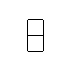
\begin{tikzpicture}
        \useasboundingbox (0,0.1) rectangle (0.2,0.3);
        \draw[step=0.2] (0,0) grid (.2,.4);
    \end{tikzpicture}
    \,\}
}
\newcommand{\gridDSet}{%
    \{\,%
    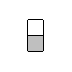
\begin{tikzpicture}
    \useasboundingbox (0,0.1) rectangle (0.2,0.3);
    \fill[gray!50] (0,0) rectangle (0.2,0.2);
    \draw[step=0.2] (0,0) grid (.2,.4);
    \end{tikzpicture}
    \,\}
}
\newcommand{\gridUSet}{%
    \{\,%
    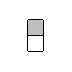
\begin{tikzpicture}
        \useasboundingbox (0,0.1) rectangle (0.2,0.3);
        \fill[gray!50] (0,0.2) rectangle (0.2,0.4);\draw[step=0.2] (0,0) grid (.2,.4);
    \end{tikzpicture}
    \,\}
}

\newcommand\ptedge[4]{
  \draw ($#1 + (0.5, -1.3) + #2$)..%
  controls ($#1 + #2 + (0.5, -1.3) + (0, -1)$)%
  and ($#3 + #4 + (0, 1) + (0.5, -0.3)$)..%
  ($#3 + #4 + (0.5, -0.3)$);
}

\newcommand{\point}[1]{%
    \begin{tikzpicture}
        \filldraw (0, 0) circle (#1);
    \end{tikzpicture}
}

\algnewcommand\algorithmicforeach{\textbf{for each}}
\algdef{S}[FOR]{ForEach}[1]{\algorithmicforeach\ #1\ \algorithmicdo}
\newcommand{\algorithmiccontinue}{\textbf{continue}}

% Paper notation : Change here should change everything in paper
\newcommand{\st}[1]{\textsf{st}\left(#1\right)}
\newcommand{\sseq}[2]{\Xi(#1,#2)}
\newcommand{\spec}[1]{\check{\mathcal{#1}}}
\newcommand{\specset}{\mathfrak{A}}
\newcommand{\specg}[1]{\mathfrak{G}\left(\check{\mathcal{#1}}\right)}
\newcommand{\sclsi}[2]{\mathcal{#1}^{\left(#2\right)}}
\newcommand{\src}{\textsf{src}}
\newcommand{\dst}{\textsf{dst}}
\newcommand{\op}{\textsf{op}}

\newcommand{\css}{\texttt{CombSpecSearcher}}
\newcommand{\tsc}{TileScope}

\newcommand{\sym}{\textsf{sym}}

\newcommand{\rev}{\textsf{r}}
\newcommand{\inv}{\textsf{i}}

\newcommand{\wordseq}[2]{#1_1 #1_2 \dotsm #1_{#2}}
\newcommand{\wordrev}[2]{#1_{#2} #1_{#2 - 1} \dotsm #1_1}
\newcommand{\wordidx}[3]{#1_{#2_1} #1_{#2_2} \dotsm #1_{#2_{#3}}}
\newcommand{\perm}[2]{\wordseq{#1}{#2}}
\newcommand{\setn}{\set{1,2,\dotsc,n}}
\newcommand{\idxset}[2]{\set{#1_1,#1_2,\dotsc,#1_{#2}}}
\newcommand{\idxord}[2]{#1_1 < #1_2 < \dotsm < #1_{#2}}

\newcommand{\sort}{\textsf{sort}}

\newcommand{\slot}{\diamond}
\newcommand{\ietrans}{\longrightarrow}
\newcommand{\iestep}[2]{\stackrel{\mathbf{#1}_{#2}}{\ietrans}}

\newcommand{\authcite}[1]{\citeauthor{#1} \cite{#1}}

%\newcommand{\idop}{\mathbf{1}^\circ}% <-- old, replaced
\DeclareFontFamily{U}{FdSymbolA}{}
\DeclareFontShape{U}{FdSymbolA}{m}{n}{<-> s * FdSymbolA-Book}{}
\DeclareSymbolFont{fdsymb}{U}{FdSymbolA}{m}{n}
\DeclareMathSymbol{\idop}{\mathrel}{fdsymb}{"6E}